\section{DownsampleGAN}

\subsection{Downsample}
\begin{frame}{Motivation}{Frequency Separation for Real World Super Resolution}
    \small
    目前超分使用已知下采样核得到的LR图像中进行训练, 得到模型会将噪声放大. 
    \begin{figure}
        \centering
        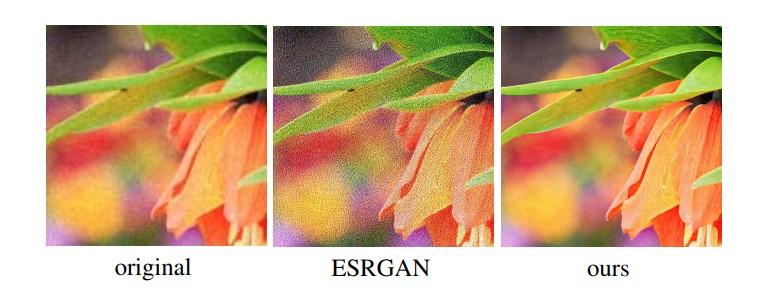
\includegraphics[height=3cm]{pic/pic0101.jpg}
        \caption{结果对比}
        \label{fig:0101}
    \end{figure}
    因此Manuel等人想在制作LR图像中引入自然图像特征
\end{frame}

\begin{frame}{Method Domain Translation}
    \small
    其做法是通过GAN的方法在下采样时学习自然图像的高频信息

    作者认为在下采样的过程中, 图像丢失了高频信息.
    \begin{figure}
        \centering
        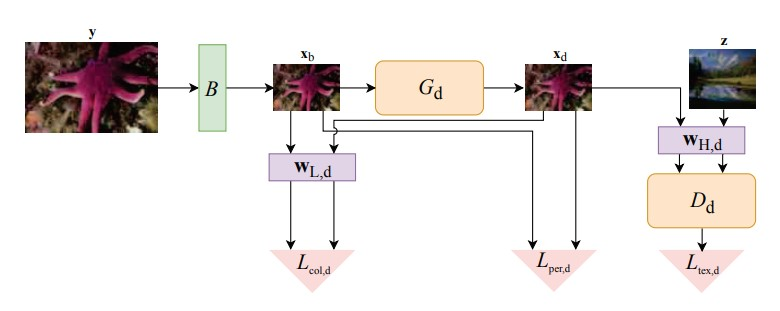
\includegraphics[height=3cm]{pic/pic0102.jpg}
        \caption{LR数据生成思路}
        \label{fig:0102}
    \end{figure}
    设计了低通滤波器$W_{L,d}$和高通滤波器$W_{H,d}$
\end{frame}

\begin{frame}{Loss Function}
    判别器损失函数设计让其只关注高频信息
    \begin{align*}
        L_{D_{d}} &=-\frac{1}{m}\sum_{i=1}^{m}mean(log D_{d}(W_{H,d})\times z^{i})) \\
        &+ mean(log(1-D_{d}(W_{H,d}\times G_{d}(x_{b}^{i}))))
    \end{align*}
    生成器的损失函数设计考虑到低频(颜色), 高频(纹理)和整体(感知)的差异.
    \begin{equation*}
        L_{G_{d}}=L_{col,d}+0.005\cdot L_{tex,d} + 0.01L_{per,d}
    \end{equation*}
\end{frame}

\subsection{Super resolution}
\begin{frame}{Super Resulotion}
    作者在超分部分改进是ESRGAN上的是加入了两个滤波器
    \begin{figure}
        \centering
        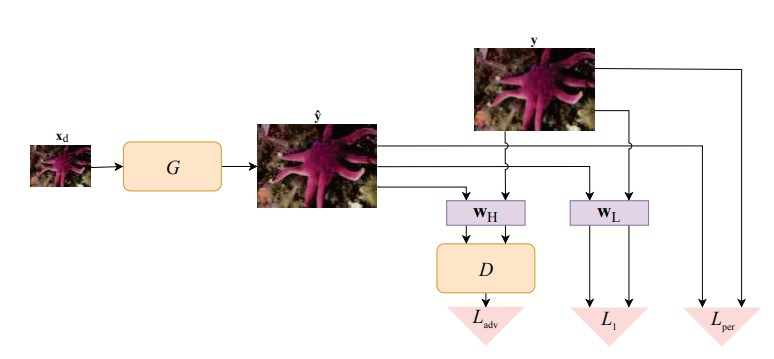
\includegraphics[height=4cm]{pic/pic0103.jpg}
        \caption{超分思路}
        \label{fig:0103}
    \end{figure}
\end{frame}

\begin{frame}{Conclusion}{Frequency Separation for Real-World Super-Resolution}
    正如论文题目Frequency Separation, 论文的思想与创新之处是将在超分过程中高低频信息的分开处理, 设计不同损失函数和网络结构, 把更多精力放在丢失的高频信息中. 在数据制作的思路上也引入了Domain Tranlation, 在网络结构中引入滤波器.
    
    该文章为2019年ICCV的SR部分的winner.
\end{frame}

% \begin{frame}{可用哨兵数据空间位置}
%     \small
%     考虑到六幅影像的范围有重叠, 只用其中一组即可
%     \begin{figure}
%         \centering
%         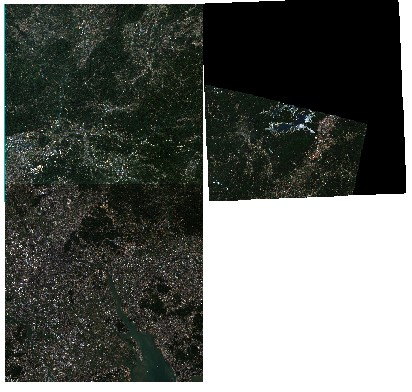
\includegraphics[width=6cm]{pic/pic0115.jpg}
%         \caption{哨兵可用重叠}
%         \label{fig:0109}
%     \end{figure}
% \end{frame}

% \begin{frame}{数据查询}
%     \begin{columns}
%         \column{0.3\textwidth}
%         \begin{itemize}
%             \item \small{对广东区域进行影像检索}
%         \end{itemize}

%         \column{0.7\textwidth}
%         \begin{figure}
%             \centering
%             % Requires \usepackage{graphicx}
%             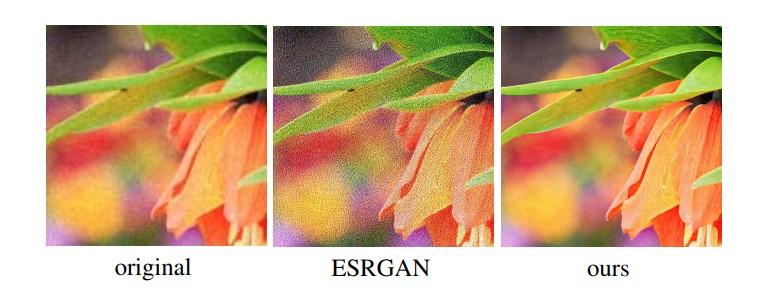
\includegraphics[width=5cm]{pic/pic0101.jpg}
%             \caption{影像查询地区}
%             \label{fig:0101}
%         \end{figure}
%     \end{columns}
% \end{frame}